\section{Bewijslast}
Dit hoofdstuk bevat de bewijslast voor de leerdoelen die in het Plan van Aanpak staan. Hier zal een apart hoofdstuk per leerdoel komen waar in diepte wordt uitgelegd waarom dit leerdoel is behaald.

\subsection{Professioneel functioneren}
Op 25 november 2014 is mijn stagedocent langs gekomen. Toen heeft ook mijn stagebegeleider een evaluatie over mij ingevuld waarmee ik wordt beoordeeld op het professionele functioneren. Het STARTT formulier hier onder zal gaan over deze evaluatie. De originele ingevulde beoordeling is te vinden in de bijlagen, Bijlage E.

\begin{tabularx}{\textwidth}{| l | X |}
\hline
\multicolumn{2}{|l|}{Academie: Academie voor Technologie \& Innovatie } \\
\hline
\multicolumn{2}{|l|}{Opleiding: HBO-ICT } \\
\hline
\multicolumn{2}{|l|}{Studentnaam: Joey Kaan \hspace{35pt} Studentnummer: 64808} \\
\hline
\multicolumn{2}{|l|}{Stagedocent: D. de Waard} \\
\hline
\multicolumn{2}{|p{\textwidth-1in}|}{Leerdoel/competentie: Professioneel functioneren.} \\
\hline
\multicolumn{2}{|l|}{Cursus: Meewerkstage \hspace{35pt} Cursuscode: CU06322} \\
\hline
\multicolumn{2}{|l|}{Datum: \today} \\
\hline
\multicolumn{2}{|l|}{Titel en nummer van bewijs/bewijzen: } \\ [50pt]
\hline
\multicolumn{2}{|l|}{Oordeel: } \\
\hline
S & Geef voorbeelden van opdrachten (situaties) waarmee je kunt aantonen dat je de competentie hebt verworven. Beschrijf kort wat er aan de hand was of om welke opdracht het ging.
\newline
\newline
De opdracht was professioneel functioneren. Ik heb bij Connect Social Business 105 dagen stage moeten lopen. Tijdens deze stage periode wordt er op een professionele manier gewerkt, dat wordt bedoeld met het professionele functioneren.
\\
\hline
T & Beschrijf de exacte rol/taak die jij had. Geef aan of het om een complexe taak ging en waaruit dat bleek. Wat moest jij doen?
\newline
\newline
Ik heb stage gelopen bij Connect Social Business als een web developer. Ik heb Content2Connect gewerkt waar alleen ik aan heb gewerkt dus waarbij ik niet hoefde te overleggen met iemand, alleen als er bijvoorbeeld een release uitgebracht moest worden dan moest ik dit overleggen met Kevin, dat is de lead developer. Naast Content2Connect heb ik ook aan Profile2Connect gewerkt. Dit project wordt samen gedaan met 2 andere mensen en hierbij moest er dus heel veel overlegd worden. Hoe het beste de architectuur van het platform opgezet kon worden, wat voor design patterns we gebruiken en wat voor algoritmes we gebruiken om bepaalde zaken op te lossen. Dat zijn een aantal voorbeelden van vragen die gesteld worden en waar over gediscussierd wordt.
\\
\hline
A & Beschrijf de activiteiten die jij achtereenvolgens hebt ondernomen in het kader van deze opdracht. Wat heb je concreet gedaan?
\newline
\newline
Tijdens het stage lopen heb ik natuurlijk een groot aantal aan activiteiten moeten doen. Een opsomming van deze activiteiten bevindt zich hieronder. Deze zullen verdeeld zijn over de opdrachten die mij toegewezen waren tijdens mijn stage periode; Content2Connect en Profile2Connect.

Voor Content2Connect:
\begin{itemize}
\item Functioneel ontwerp maken Content2Connect; gesprek met opdrachtgever (Paul)
\item Nadenken over technische architectuur Content2Connect
\item Uitwerken prototype Content2Connect
\item Uitwerking prototype bespreken met lead developer (Kevin)
\item Feedback verwerken van lead developer
\item Uitwerking prototype bespreken met opdrachtgever (Paul)
\item Feedback verwerken van opdrachtgever
\item Daadwerkelijk Content2Connect gaan ontwerpen \& programmeren
\item Tests schrijven voor Content2Connect
\end{itemize}

Voor Profile2Connect:
\begin{itemize}
\item Samen met andere twee collega's structuur bespreken van Profile2Connect
\item Functionaliteit duidelijk krijgen voor Profile2Connect; gesprek met opdrachtgever (Jeroen)
\item Uitwerken functionaliteit in prototype
\item Klaarmaken voor release; tests schrijven en afronden development
\item Functionaliteit volgende release duidelijk krijgen voor Profile2Connect; gesprek met opdrachtgever (Jeroen)
\end{itemize}
\\
\hline
R & Beschrijf het resultaat van de opdracht en hoe de betrokken en er op reageerden. Wat is er vervolgens met dat resultaat gebeurd?
\newline
\newline
Alhoewel bij de activiteiten concrete opdrachten worden beschreven is het resultaat van dit leerdoel niet zozeer iets fysieks. Het is meer een gevoel dat mensen bij de persoon hebben en op basis van dit gevoel kunnen ze een evaluatie invullen.
Kevin, de lead developer, heeft dus een evaluatie ingevuld met zijn mening over hoe ik tijdens mijn stage professioneel heb gefunctioneerd. De evaluatie is te zien in de bijlage.
\\
\hline
R & Wat heb je ervan geleerd? Wat zou je volgende keer anders aanpakken en waarom?
\newline
\newline
Uit de evaluatie blijkt dat ik op eigenlijk alle punten boven het gemiddelde zit, alleen bij nauwkeurigheid en stiptheid ben ik gemiddeld. Hoewel ik natuurlijk aan alle punten zal blijven werken heb ik wel geleerd dat ik nauwkeuriger en stipter moet gaan werken, dit is natuurlijk een zeer belangrijke kwaliteit van een developer. Wat betreft mijn mening over de evaluatie, ik vind dat Kevin mij heel goed heeft ingeschat. Ik heb vaak moeite met het nauwkeurig werken omdat ik altijd die druk voel dat het snel af moet komen. Vaak is de oplossing die even snel bedacht wordt wel functioneel maar niet zozeer dat dit de beste oplossing is. Ik denk dat ik wat vaker naar mijn gemaakte code zou moeten kijken en deze dan reviewen om te kijken of er toch niet iets is wat ik zou kunnen verbeteren.
\\
\hline
T & Geef een voorbeeld van een andere situatie waarin je deze competentie kunt toepassen
\newline
\newline
Deze competentie is natuurlijk te gebruiken bij elke situatie in het bedrijfsleven. Het moet altijd prioriteit hebben dat je professioneel omgaat met collega's en opdrachtgevers. Ik weet nu waar mijn plus punten zijn en waar mijn min punten zijn, omdat ik deze nu weet kan ik deze van te voren aangeven aan mijn collega's zodat ze op de hoogte zijn van eventuele tekortkomingen die ik kan vertonen. Zo weten ze ook wat ze van mij kunnen verwachten en is het ook makkelijker in te schatten hoeveel tijd een bepaald project zal kosten.
\\
\hline
\end{tabularx}

\subsection{Facebook API}

\clearpage

\subsection{Meteor, een JavaScript framework}
Het leerdoel dat hierbij hoort: Meteor leren kennen door middel van een applicatie te maken die real-time informatie weergeeft over een klant’s social media kanalen aan meerdere eind-gebruikers, dit wordt verwezenlijkt door Meteor’s collections en het publish-subscribe pattern te gebruiken.

Normaliter deed ConnectSB alles met PHP en dan vooral het Symfony framework. Profile2Connect was een speciaal geval, het moest mogelijk zijn om heel veel data op te slaan en dynamisch velden toe te voegen aan de database. Door deze speciale eisen is er toen gekozen voor Meteor. Meteor is een JavaScript framework waarmee het mogelijk is om de backend evenals de frontend in JavaScript te programmeren. Meteor is zeer recent, op het moment van schrijven is Meteor nog in beta, versie 0.9.3.1 om precies te zijn. Dit brengt natuurlijk wel de nodige problemen met zich mee, weinig documentatie en vooral veel kans op performance issues. Meteor zelf maakt gebruik van het publish-subscribe pattern om zogenaamde collecties van de server naar de client beschikbaar te maken. Deze collecties zijn niets anders als tabellen, op de server worden ze gepublished en op de client kun je deze dan ontvangen (subscriben). Op de server kun je aangeven welke velden er wel beschikbaar worden gemaakt en welke niet, wegens performance issues is het natuurlijk beter om alleen de velden beschikbaar te maken die nodig zijn.

\newline

Meteor beschikt ook over iets wat heet latency compensation. Als een eind-gebruiker iets veranderd ziet deze eind-gebruiker de verandering meteen. Meteor stuurt dit daarna op, ontvangt de respons, vergelijkt dit met de client en voert daarna de echte wijziging door. De eind-gebruiker ziet hier niets van, tenzij er iets mis gaat in het proces van vergelijken maar dat gebeurt nagenoeg nooit. Met een platform waar heel veel data in staat kan het wel eens zijn dat de database verbinding wat aan de trage kant wordt, Meteor zorgt ervoor dat hoe langzaam de verbinding ook wordt de eind-gebruiker hier maar minimaal mee te maken zal hebben.

\newline

Profile2Connect wordt gemaakt door mij en nog een medewerker van ConnectSB, Jimmy. Ik ben verantwoordeljik voor de homepage van Profile2Connect welke er als volgt uitziet:

\begin{center}
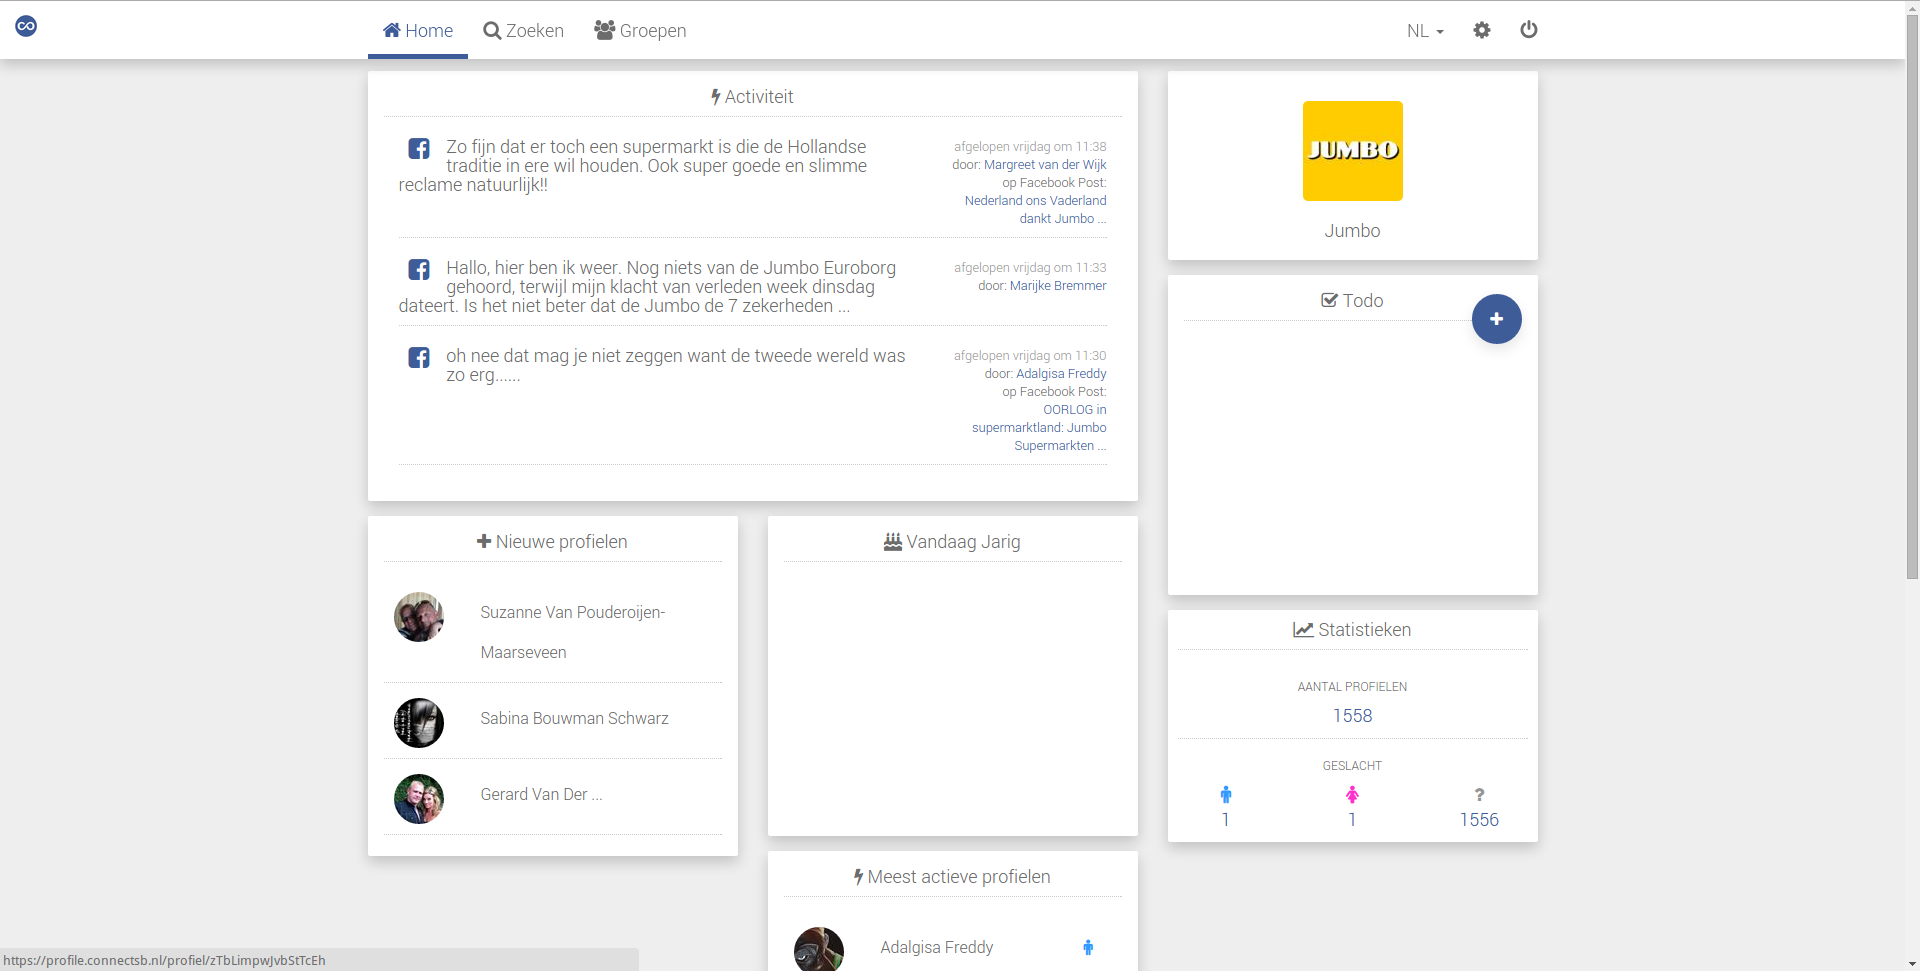
\includegraphics[scale=0.2]{profile2connect}
\end{center}


De gegevens die te zien zijn op deze pagina komen van verschillende publicaties. Zo zie je bijvoorbeeld een logo van de op dit moment ingelogde klant(rechts boven in), de updates (links boven in) en dan nog een aantal overige categoriën zoals nieuwe profielen en meest actieve profielen. Al deze categoriën zijn allemaal aparte publicaties, dit wordt gedaan omdat je dan nooit meer data beschikbaar hebt op de client dan dat je nodig hebt. Het optellen van de totalen wordt ook op de server gedaan, je wilt natuurlijk niet alle profielen van een klant op de welkomst pagina beschikbaar maken. Hierdoor zou de applicatie heel lang kunnen doen over het laden, omdat hij al deze profielen uit de database zou moeten halen.

\clearpage

\subsection{Versiebeheer}
Het desbetreffende leerdoel is: Versiebeheer volgens de Gitflow workflow gebruiken zodat er altijd een fout vrije en uitrolbare versie van de applicatie beschikbaar is en als er een fout optreedt deze snel weer ongedaan gemaakt kan worden door naar een vorige versie terug te keren.

\begin{tabularx}{\textwidth}{| l | X |}
\hline
\multicolumn{2}{|l|}{Academie: Academie voor Technologie \& Innovatie } \\
\hline
\multicolumn{2}{|l|}{Opleiding: HBO-ICT } \\
\hline
\multicolumn{2}{|l|}{Studentnaam: Joey Kaan \hspace{35pt} Studentnummer: 64808} \\
\hline
\multicolumn{2}{|l|}{Stagedocent: D. de Waard} \\
\hline
\multicolumn{2}{|p{\textwidth-1in}|}{Leerdoel/competentie: Versiebeheer volgens de Gitflow workflow gebruiken zodat er
altijd een fout vrije en uitrolbare versie van de applicatie beschikbaar is en als
er een fout optreedt deze snel weer ongedaan gemaakt kan worden door naar
een vorige versie terug te keren.} \\
\hline
\multicolumn{2}{|l|}{Cursus: Meewerkstage \hspace{35pt} Cursuscode: CU06322} \\
\hline
\multicolumn{2}{|l|}{Datum: \today} \\
\hline
\multicolumn{2}{|l|}{Titel en nummer van bewijs/bewijzen: } \\ [50pt]
\hline
\multicolumn{2}{|l|}{Oordeel: } \\
\hline
S & Geef voorbeelden van opdrachten (situaties) waarmee je kunt aantonen dat je de competentie hebt verworven. Beschrijf kort wat er aan de hand was of om welke opdracht het ging.
\newline
\newline
De opdracht was Content2Connect. Deze was zo ver dat er een versie 1.0 kon worden uitgebracht. \\
\hline
T & Beschrijf de exacte rol/taak die jij had. Geef aan of het om een complexe taak ging en waaruit dat bleek. Wat moest jij doen?
\newline
\newline
Mijn rol was het klaarmaken van Content2Connect voor de release, Content2Connect te releasen en daarna deze ook te beheren. Met beheren wordt bedoeld of de release goed is gelukt, of alle functies ook werken op de productie server. Zo niet dan zal hier wat aanpassingen aan gedaan moeten worden. Hiernaast moet ook de feedback van klanten en van de interne gebruikers van ConnectSB worden verwerkt en bugs gefixed worden naarmate deze worden gevonden.
\\
\hline
A & Beschrijf de activiteiten die jij achtereenvolgens hebt ondernomen in het kader van deze opdracht. Wat heb je concreet gedaan?
\begin{itemize}
\item Functionaliteit voor Content2Connect afmaken.
\item Online zetten voor testen op test omgeving.
\item Test periode doorlopen waarbij getest wordt door management en community management.
\item Feedback verwerken van de test periode.
\item Online zetten op de productie omgeving.
\item Bugs gefixed die gaande weg ontdekt werden.
\item Nieuwe branch aangemaakt met de volgende naam: hotfix-testbugs.
\item Bugs opgelost in deze branch.
\item Hotfix-testbugs branch gemerged met master branch
\end{itemize}
\\
\hline
R & Beschrijf het resultaat van de opdracht en hoe de betrokken en er op reageerden. Wat is er vervolgens met dat resultaat gebeurd?
\newline
\newline
Het resultaat was een volledig werkende versie van  Content2Connect, de eerste dag hadden er al twee klanten gebruik gemaakt van het platform en dit was allemaal succesvol verlopen. De klanten waren heel enthousiast over het platform, het werkte heel prettig en het was vooral heel overzichtelijk.
\\
\hline
R & Wat heb je ervan geleerd? Wat zou je volgende keer anders aanpakken en waarom?
\newline
\newline
Tijdens het klaarmaken van Content2Connect voor de release heb ik geleerd dat het continue testen heel erg belangrijk is. Bij ConnectSB is er nog maar sinds kort de regel dat er tests geschreven moeten worden en Content2Connect had deze tests nog niet. In Content2Connect worden er verschillende notificaties verstuurd met hierbij bijbehorende emails. De emails werden soms wel verzonden en soms niet bleek na de test periode. Als hiervoor tests geschreven waren had ik heel erg gemakkelijk kunnen zien waar de fout zat. Zo heb ik toen nog wel tests geschreven voor de email functie en hiermee kon ik dus heel gemakkelijk ook zien waar de fout zat.
\\
\hline
T & Geef een voorbeeld van een andere situatie waarin je deze competentie kunt toepassen
\newline
\newline
Deze competentie is eigenlijk te gebruiken gedurende de hele levensduur van de software. De Gitflow workflow gaat niet alleen over software die al in gebruik genomen wordt. Het is een workflow die het makkelijk maakt om aan aparte features te werken zonder dat de toestand van het development werk en de toestand van de code die productie gereed is wordt aangetast.
\\
\hline
\end{tabularx}

\newline

Voor Content2Connect moesten een aantal belangrijke fixes gebeuren, deze hadden hoge prioriteit. Deze komen volgens de Gitflow workflow dan op zogenaamde feature branches. Er is geen speciale conventie voor hoe deze feature branches moeten heetten maar heel veel bedrijven houden de volgende conventie aan: feature/[feature-naam], dit heb ik dus ook gedaan. Mijn branch voor deze belangrijke fixes heet daarom ook feature/important-fixes. Bij ConnectSB wordt gewerkt met Redmine en hierbij kan er prioriteit gegeven worden aan bepaalde issues. Deze hoge prioriteit komt dus ook van Redmine.

Voor een grote hoeveelheid met kleine issues is het in mijn belevenis beter om een branch te maken die deze allemaal bevat. Veel bedrijven houden zich ook aan het aanmaken van één branch voor elke issue, maar dit is naar mijn idee geen goed idee. Als een issue natuurlijk best wel uitgebreid is en je waarschijnlijk kleine taken zult hebben is dit een goed idee, maar als je één issue moet doen die hooguit 5 minuten duurt is dit het natuurlijk niet echt waard.

\newline

Ik moest in Content2Connect bij het overzicht van één bestelling de titel toevoegen van de bestelling. Hiervoor wordt er dan een branch gemaakt genaamd feature/change-\#2318 want de issue heet op Redmine Change \#2318. Change is dan de categorie en \#2318 is het nummer van de issue.

Dit is dus nu gedaan voor elke issue die op Redmine stond. Deze branches komen eigenlijk nooit op de centrale repository. Deze kunnen gepusht worden als dat nodig is, bijvoorbeeld als iemand mee moet helpen om aan een bepaalde feature mee te werken. Features zullen meest van de tijd, in ieder geval in mijn situatie, werk bevatten voor één persoon dus de feature branches hoeven dan nooit gepusht te worden.

\newline

Vandaag is er een release voor Content2Connect uitgebracht. Dit is versie v0.9, hier wordt dan een tag voor aangemaakt op de master en dan kan deze in productie gezet worden.

Gitflow workflow werkt vooral heel goed als je bijvoorbeeld bezig bent aan nieuwe functionaliteit, maar je baas zegt dat er even snel wat anders moet gebeuren. Je maakt een nieuwe feature branch aan, commit daar alles op. Deze merge je dan met de develop branch en indien nodig kan deze naar master voor een nieuwe release. Alle changes waar je dan eerst mee bezig was kun je dan heel gemakkelijk weer.

\clearpage

\subsection{Functioneel ontwerp}

